\subsection{Pianificazione temporale degli incrementi}
Il periodo 2 della fase di Progettazione di Dettaglio e di Codifica e della fase di Validazione e Collaudo sono in gran parte dedicate alla progettazione e all'implementazione dei requisiti degli incrementi.
Gli incrementi vengono suddivisi temporalmente come elencati di seguito.

\subsubsection{Incrementi con requisiti obbligatori}
\begin{itemize}
	\item Incremento 1: 2020-04-08 $\rightarrow$ 2020-04-12 (5 giorni);
	\item Incremento 2: 2020-04-13 $\rightarrow$ 2020-04-17 (5 giorni);
	\item Incremento 3: 2020-04-18 $\rightarrow$ 2020-04-23 (6 giorni);
	\item Incremento 4: 2020-04-24 $\rightarrow$ 2020-05-01 (8 giorni);
	\item Incremento 5: 2020-05-02 $\rightarrow$ 2020-05-06 (5 giorni).
\end{itemize}

\subsubsection{Incrementi con requisiti desiderabili e opzionali}
\begin{itemize}
	\item Incremento 6: 2020-05-23 $\rightarrow$ 2020-05-28 (6 giorni);
	\item Incremento 7: 2020-05-29 $\rightarrow$ 2020-05-31 (3 giorni);
	\item Incremento 8: 2020-06-01 $\rightarrow$ 2020-06-05 (5 giorni);
	\item Incremento 9: 2020-06-06 $\rightarrow$ 2020-06-10 (5 giorni);
\end{itemize}

%PAGINA ORIZZONTALE
\newpage
\paperwidth=\pdfpageheight
\paperheight=\pdfpagewidth
\pdfpageheight=\paperheight
\pdfpagewidth=\paperwidth
\headwidth=\textheight

\begingroup 
\vsize=\textwidth
\hsize=\textheight

\pagestyle{empty}
\begin{figure}[h]
	\centering
	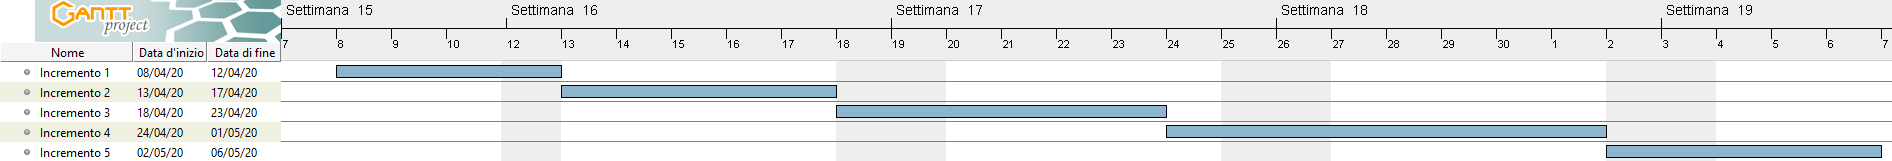
\includegraphics[height = 4cm, width = 24.5cm]{Sezioni/Immagini/DiagrammiGantt/PianificazioneTemporaleIncrementi.png}
	\caption{Diagramma di Gantt degli incrementi del Periodo 2 della Fase di Progettazione di Dettaglio e Codifica}
\end{figure}

\begin{figure}[h]
	\centering
	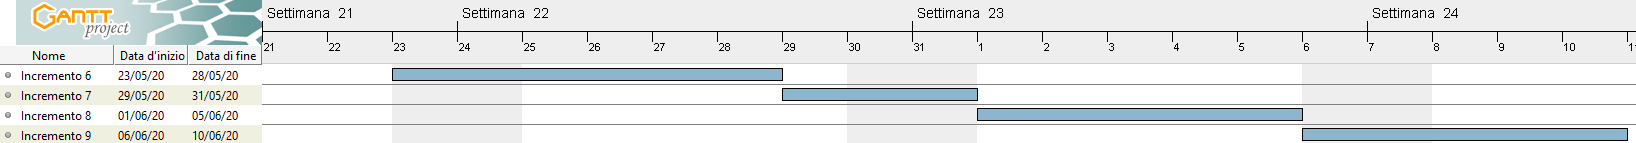
\includegraphics[height = 4cm, width = 24.5cm]{Sezioni/Immagini/DiagrammiGantt/PianificazioneTemporaleIncrementi2.png}
	\caption{Diagramma di Gantt degli incrementi del Periodo 2 della Fase di Validazione e Collaudo}
\end{figure}

\textwidth=\hsize
\textheight=\vsize

\endgroup
\newpage
\paperwidth=\pdfpageheight
\paperheight=\pdfpagewidth
\pdfpageheight=\paperheight
\pdfpagewidth=\paperwidth
\headwidth=\textwidth